% !TeX program = xelatex
\documentclass[9pt]{beamer}
\usepackage{xcolor}
\definecolor{orange}{HTML}{EF767A}
\definecolor{red}{HTML}{AC454A}
\definecolor{brown}{HTML}{EAD296}
\definecolor{darkgrey}{HTML}{313630}
\usefonttheme{professionalfonts} % using non standard fonts for beamer
\usefonttheme{serif} % default family is serif
\usepackage{fontspec}
\usepackage{setspace}
\usepackage{natbib}
\usepackage{animate}
\usepackage{graphicx}
%\usepackage[T1]{fontenc}

\bibliographystyle{abbrv}
%\setmainfont{Liberation Serif}
%\setmainfont{Liberation Serif}
\setmainfont{Comfortaa}
%\usepackage[T1]{fontenc}

\setbeamercolor{frametitle}{bg=orange,fg=white}
\setbeamercolor{author in head/foot}{bg=orange,fg=white}

%\setbeamerfont{page number}{size=\Huge}

%\setbeamertemplate{itemize items}[circle]
\useinnertheme{circles}
\setbeamercolor{palette primary}{bg=orange,fg=white}
%\setbeamercolor{palette secondary}{bg=red,fg=white}
\setbeamertemplate{itemize item}{\color{darkgrey}$\circ$}
\setbeamercolor{structure}{fg=red} % itemize, enumerate, etc

%\setbeamercolor{section in head/foot}{bg=red}
\setbeamercolor{title}{fg=orange} %, bg=brown
\setbeamercolor{author}{fg=darkgrey}
\setbeamercolor{institute}{fg=darkgrey}
\setbeamercolor{date}{fg=darkgrey}
%\setbeamercolor{normal text}{fg=darkgrey}
\makeatletter
\setbeamertemplate{headline}{%
	\usebeamercolor[bg]{frametitle}\rule{\textwidth}{1cm}
}
\setbeamerfont{title}{size=\LARGE}
\setbeamerfont{institute}{size=\normalsize}
\renewcommand*{\bibfont}{\scriptsize}


\setbeamertemplate{frametitle}{%
	\vskip-1cm%
	\begin{minipage}[c][\headheight][c]{\textwidth}%
		\usebeamerfont{frametitle}
		\strut\insertframetitle\par
		{%
			\ifx\insertframesubtitle\@empty%
			\else%
			{\usebeamerfont{framesubtitle}\usebeamercolor[fg]{framesubtitle}\strut\insertframesubtitle\par}%
			\fi
		}%      
		\vspace*{0.05cm}
	\end{minipage}%
	\vskip-0.1em
}
%\setbeamertemplate{footline}{%
%	\leavevmode%
%	\hbox{\begin{beamercolorbox}[wd=\paperwidth,ht=4.5ex,dp=3.125ex]{author in head/foot}%
%			\usebeamerfont{author in head/foot} bar
%	\end{beamercolorbox}}%
%	\vskip0pt%
%}
\makeatother


\title{Unsupervised Learning \\
	of Disentangled and Interpretable Representations from Sequential Data}
\author{Wei-Ning Hsu, Yu Zhang, and James Glass\\Talk by Stefan Wezel}
\institute{Explainable Machine Learning}

\date{\today}


%\setbeamertemplate{sidebar right}{}
%\setbeamertemplate{footline}{%
%	\hfill\usebeamertemplate***{navigation symbols}
%	\hspace{1cm}\insertframenumber{}}
\setbeamerfont{page number in head/foot}{size=\small}
    \setbeamertemplate{footline}{%
	\raisebox{5pt}{\makebox[\paperwidth]{\hfill\makebox[10pt]{\scriptsize\insertframenumber}}}}
\setbeamertemplate{navigation symbols}{}
%\onehalfspacing
\setstretch{1.3}
\begin{document}
	

\setbeamercolor{background canvas}{bg=white}
\setbeamercolor{normal text}{fg=darkgrey}
\usebeamercolor[fg]{normal text}
\begin{frame}[plain]
	\titlepage
\end{frame} 



\setbeamercolor{background canvas}{bg=white}
\setbeamercolor{normal text}{fg=darkgrey}
\usebeamercolor[fg]{normal text}
\setbeamertemplate{itemize item}{\color{darkgrey}$\circ$}
\begin{frame}
\frametitle{Overview}
%\framesubtitle{}
\begin{itemize}%\setlength\itemsep{1.5em}
	\item Introduction
	\item What are disentangled representations (intuition)
	\item Why disentangled representations
	\item Formal description of disentangled representations
	\item SequentialVAE
	\item Did they achieve disentanglement?
	\item Other approaches and challenges
\end{itemize}
\end{frame} 



\setbeamercolor{background canvas}{bg=white}
\setbeamercolor{normal text}{fg=darkgrey}
\usebeamercolor[fg]{normal text}
\setbeamertemplate{itemize item}{\color{darkgrey}$\circ$}
\begin{frame}
\frametitle{Overview}
%\framesubtitle{}
\begin{itemize}%\setlength\itemsep{1.5em}
	\item Using Sequential VAE ( -> Unsupervised representation learning)
	\item Represent information from different temporal scales in corresponding latent subspaces
	\item Claim that they achieve disentanglement with respect to sequence (speaker) and segment (content) information
	\item would mean that those latent variables then can be used separately
	\begin{itemize}
		\item speaker verification
		\item denoising
		\item ...
	\end{itemize}
\end{itemize}
\end{frame} 




\setbeamercolor{background canvas}{bg=white}
\setbeamercolor{normal text}{fg=darkgrey}
\usebeamercolor[fg]{normal text}
\setbeamertemplate{itemize item}{\color{darkgrey}$\circ$}
\begin{frame}
\frametitle{What is disentanglement?}
\framesubtitle{Intuition}
	\begin{itemize}%\setlength\itemsep{1.5em}
	\item encode distinct generating factors in separate subsets of latent space dimensions
	%\item i.e. color as one subspace, translation, as another
	%\item The exact definition is often discussed, we will have a look at a proposed one
	\end{itemize}
%\animategraphics[autoplay,loop,width=\linewidth/2]{10}{disentangled_scene-}{0}{19}
\begin{figure}
	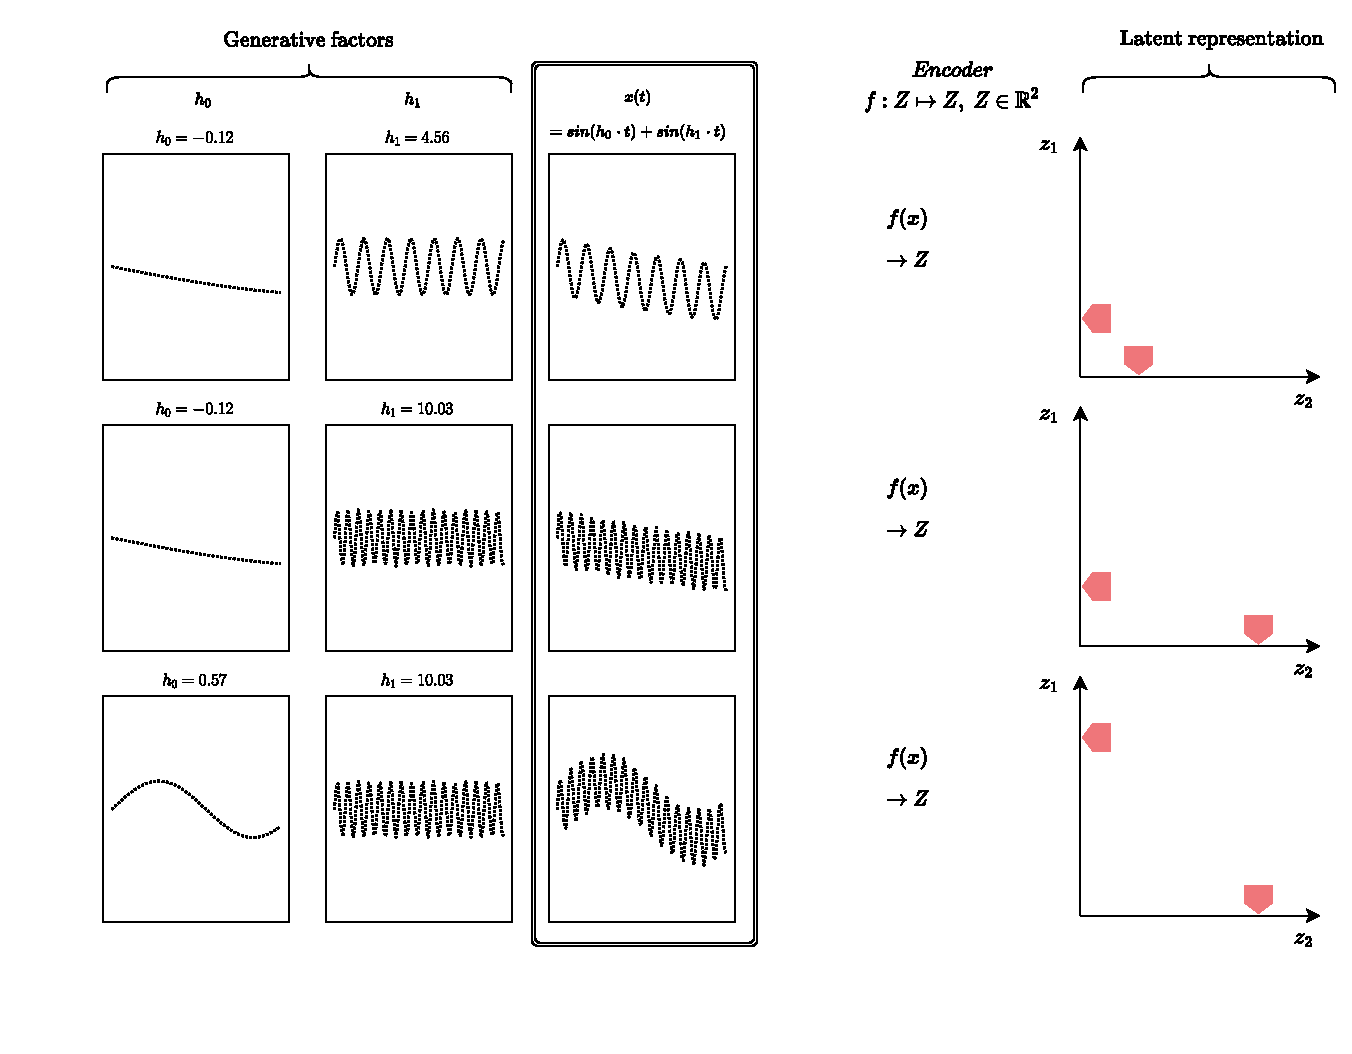
\includegraphics[width=.95\linewidth]{figures/intution_3x3.pdf}
	%\caption{World states are determinded by two generative factors, a change in those is reflected in the two corresponding latent variables, our $f$ maps to}
\end{figure}
\end{frame} 





\setbeamercolor{background canvas}{bg=white}
\setbeamercolor{normal text}{fg=darkgrey}
\usebeamercolor[fg]{normal text}
\setbeamertemplate{itemize item}{\color{darkgrey}$\circ$}
\begin{frame}
\frametitle{Why learn disentangled representations?}
\framesubtitle{Motivation}
\begin{itemize}%\setlength\itemsep{1.5em}
	\item Gives us an exact idea, of what variables were used, to come to a result
	\begin{itemize}
			\item Fairness in ML (exact)
			\item Explainability/Interpretability
			\item Overall, a model just becomes more usable if latent variables carry semantic meaning		
	\end{itemize}

\end{itemize}
\end{frame} 



\setbeamercolor{background canvas}{bg=white}
\setbeamercolor{normal text}{fg=darkgrey}
\usebeamercolor[fg]{normal text}
\setbeamertemplate{itemize item}{\color{darkgrey}$\circ$}
\begin{frame}
\frametitle{Disentangled Representations Formally}
\framesubtitle{A field-trip to group theory: important concepts}
\begin{itemize}%look at simple example here
	\item Group
	\begin{itemize}
		\item tuple of operation and set
		\item set is closed under operation, there is identity element, and inverse for every element, associativity
	\end{itemize}
	\item Symmetry group
	\begin{itemize}
		%\item A bit more general
		\item Group action, that leaves object (defined through set/sets) invariant
		%\item has group operation (i.e. composition)
		%\item set of transformations on some object that preserve object
		%For example: If we shift signal, it's still the signal... 
	\end{itemize}
	\item Group action
	\begin{itemize}
		\item Actions are results of symmetry transformations of set (i.e. set of changed order)
		%\item $\cdot :G \times X \mapsto X$
	\end{itemize}
	\item Direct product
	\begin{itemize}
		\item $G = G_1 \times ... \times G_n$
		\item Group conditions must hold for group and each subgroup
	\end{itemize}
\end{itemize}
\end{frame} 



\setbeamercolor{background canvas}{bg=white}
\setbeamercolor{normal text}{fg=darkgrey}
\usebeamercolor[fg]{normal text}
\setbeamertemplate{itemize item}{\color{darkgrey}$\circ$}
\begin{frame}
\frametitle{Disentangled Representations Formally}
\framesubtitle{A field-trip to group theory: What is disentanglement in terms of group theory?}
\begin{itemize}%\setlength\itemsep{1.5em}
	\item Disentangled group actions
	\begin{itemize}
		\item Result of transformations that only change certain aspect of world, but leave others invariant
	\end{itemize}
	\item Assuming $G$ can be decomposed into direct product symmetry subgroups $G_i$
	\item We want mapping $f:W \mapsto Z$
	\item Symmetry $G$ on $W$ should be preserved in $Z$, $G \times Z \mapsto Z$
	\begin{itemize}
		\item $g \cdot f(w) = f(g\cdot w)$ -> equivariant map
	\end{itemize}
\end{itemize}
\end{frame} 


\setbeamercolor{background canvas}{bg=white}
\setbeamercolor{normal text}{fg=darkgrey}
\usebeamercolor[fg]{normal text}
\setbeamertemplate{itemize item}{\color{darkgrey}$\circ$}
\begin{frame}
\frametitle{Disentangled Representations Formally}
\framesubtitle{A field-trip to group theory: What is disentanglement in terms of group theory?}
\begin{itemize}%\setlength\itemsep{1.5em}
	\item Representation is disentangled if
	\begin{itemize}
		%\item action $\cdot : G \times Z \mapsto Z$
		\item equivariant map $f:W \mapsto Z, g \cdot f(w) = f(g\cdot w) \forall g \in G,w \in W$ % %between actions on $W$ and $Z$
		\item such a map would split $Z$ into independent subspaces, thus satisfying:
		\begin{itemize}
			%representation reflects transformation applied to input
			\item Decomposition $Z = Z_{1} \times ... \times Z_{n}$
			\item where $Z_{i}$ is only affected by transformations $G_i$ in $W$% ($G_{j\neq i}$)
			\item and $Z_i$ invariant to all $G_{j \neq i}$ in $W$ %$Z_{warped}$ is only affected by warps in $W$ ($G_{warps}$) % G acts on W this affects Z
			\item Thus each subspace $Z_i$ can be transformed ONLY by the corresponding symmetry of $W$%(like shift or warp independently)
		\end{itemize}
		%\item action $\cdot$ on $Z$ is disentangled according to definition from before
	\end{itemize}
	%\item There may be more criteria (preserving group structure, isomorphisms, ...) but for the intuition this is sufficient
	%\item (Note that much prior knowledge about our world was injected here)
\end{itemize}
\end{frame} 



\setbeamercolor{background canvas}{bg=white}
\setbeamercolor{normal text}{fg=darkgrey}
\usebeamercolor[fg]{normal text}
\setbeamertemplate{itemize item}{\color{darkgrey}$\circ$}
\begin{frame}
\frametitle{Disentangled Representations Formally}
\framesubtitle{A field-trip to group theory: Disentangle our example formally}
\begin{itemize}%\setlength\itemsep{1.5em}
	\item signal $x(t) = sin(h_0 \cdot t) + sin(h_1 \cdot t)$ with $h_0 \sim \mathcal{N}(0,1),\;h_1 \sim \mathcal{N}(5,1);$
	\item The set of possible values for $h_0, h_1$ make up our $W$
	\item The group of symmetries acting on this $W$ decompose into $G = G_{h_0} \times G_{h_1}$
	\item We want to find an equivariant map $f:W\mapsto Z$ with $Z \in \mathbb{Z}^2$
	\item so that changes of $h_0$ result ONLY in changes in $z_0$ and changes of $h_1$ ONLY in $z_2$
	\item Note, that this requires prior knowledge of generating factors in our world
\end{itemize}
\end{frame} 


\setbeamercolor{background canvas}{bg=white}
\setbeamercolor{normal text}{fg=darkgrey}
\usebeamercolor[fg]{normal text}
\setbeamertemplate{itemize item}{\color{darkgrey}$\circ$}
\begin{frame}
\frametitle{Disentangled Representations Formally}
\framesubtitle{A field-trip to group theory: Disentangle our example formally}
\begin{figure}
	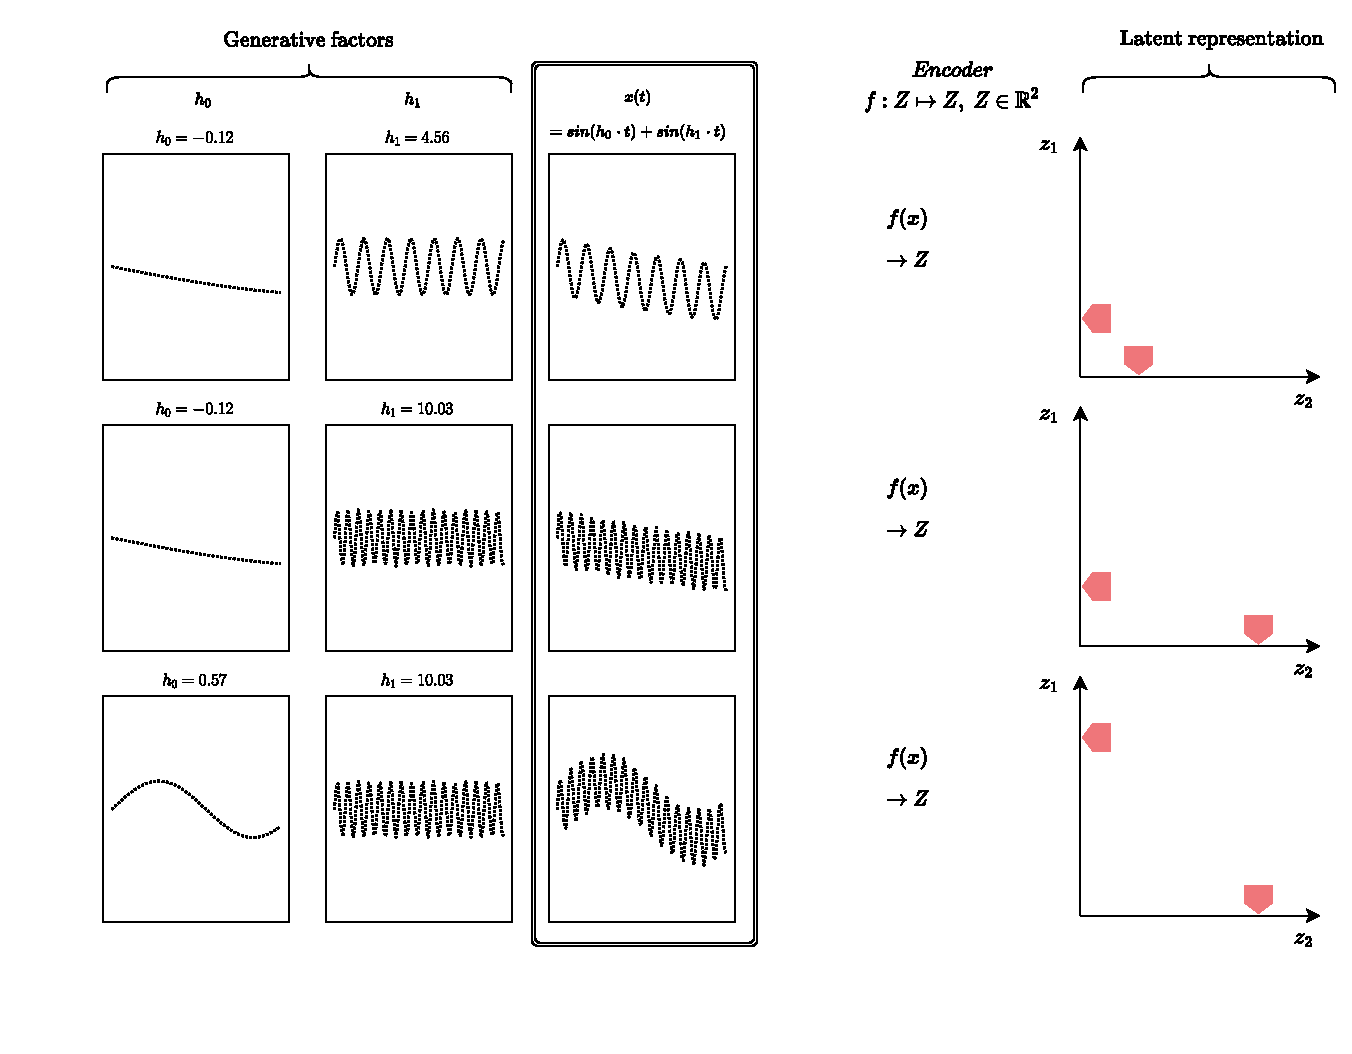
\includegraphics[width=1\linewidth]{figures/intution_3x3.pdf}
\end{figure}
\end{frame} 


\setbeamercolor{background canvas}{bg=white}
\setbeamercolor{normal text}{fg=darkgrey}
\usebeamercolor[fg]{normal text}
\setbeamertemplate{itemize item}{\color{darkgrey}$\circ$}
\begin{frame}
\frametitle{Back to the paper}
\framesubtitle{Did they achieve disentanglement?}
\begin{itemize}
	\item Disentangled with respect to what decomposition?
	\item Assuming there is a decomposition $G = G_{sequence} \times G_{segment}$
	\item This should be reflected in $Z= (z_1, z_2)$
	\item They propose to store sequence information in $z_2$ and segment information in $z_1$
	\item Thus, they need to find an equivariant map $f:W\mapsto Z$, so that $z_1$ is only affected by actions on $G_{sequence}$ and vice versa
\end{itemize}
\end{frame} 



\setbeamercolor{background canvas}{bg=white}
\setbeamercolor{normal text}{fg=darkgrey}
\usebeamercolor[fg]{normal text}
\setbeamertemplate{itemize item}{\color{darkgrey}$\circ$}
\begin{frame}
\frametitle{FHVAE}
\framesubtitle{Encoder}
\begin{figure}
	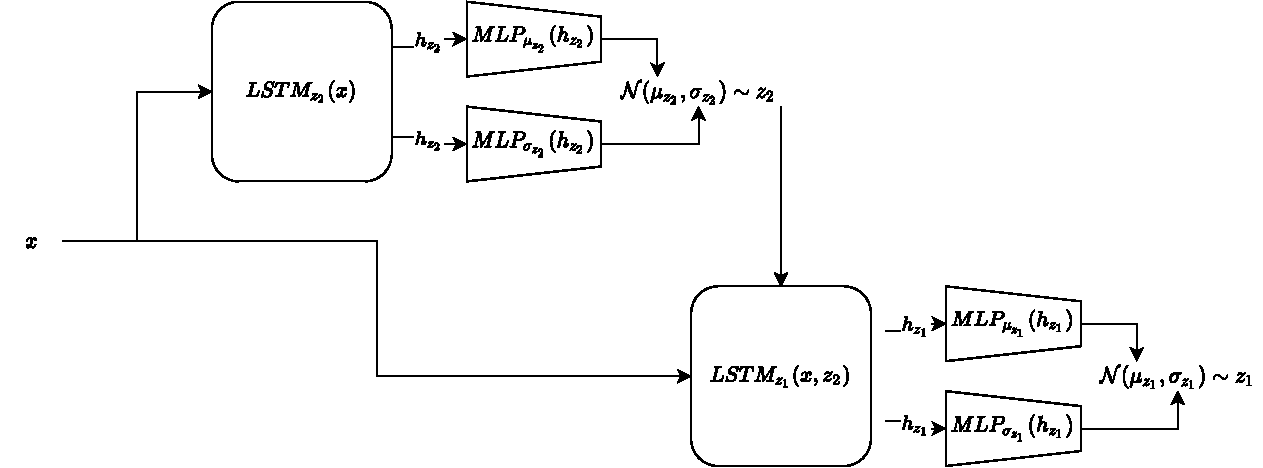
\includegraphics[width=1\linewidth]{figures/fhvae_encoder.pdf}
\end{figure}
\end{frame} 

\setbeamercolor{background canvas}{bg=white}
\setbeamercolor{normal text}{fg=darkgrey}
\usebeamercolor[fg]{normal text}
\setbeamertemplate{itemize item}{\color{darkgrey}$\circ$}
\begin{frame}
\frametitle{FHVAE}
\framesubtitle{Decoder}
\begin{figure}
	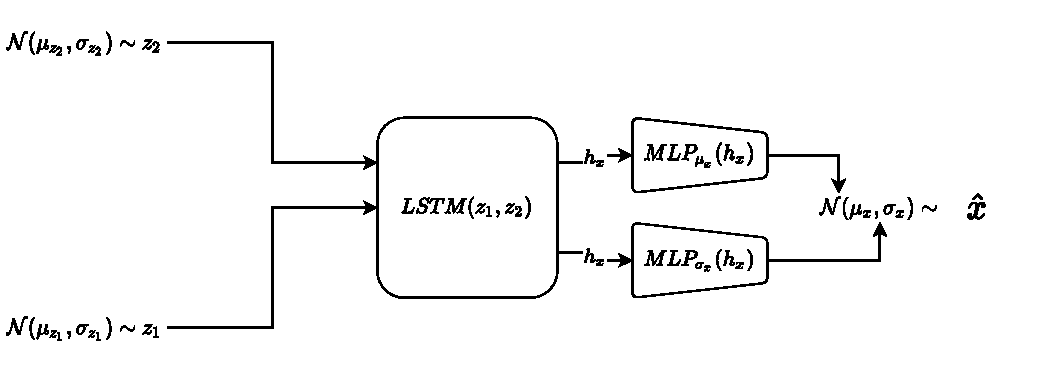
\includegraphics[width=.8\linewidth]{figures/fhvae_decoder.pdf}
\end{figure}
\end{frame} 

\setbeamercolor{background canvas}{bg=white}
\setbeamercolor{normal text}{fg=darkgrey}
\usebeamercolor[fg]{normal text}
\setbeamertemplate{itemize item}{\color{darkgrey}$\circ$}
\begin{frame}
\frametitle{Back to the paper}
\framesubtitle{How did they do it?}
\begin{itemize}
	\item regularize z2 by sequence dependent prior (lookup table of s-vectors)
	\item and z1 by sequence independent prior 
	\item optimize latent space at segment level
	%\item optmization is outsourced to $\mu_2$
\end{itemize}
%\begin{figure}
%	\includegraphics[width=.7\linewidth]{}
%\end{figure}
\end{frame} 



\setbeamercolor{background canvas}{bg=white}
\setbeamercolor{normal text}{fg=darkgrey}
\usebeamercolor[fg]{normal text}
\setbeamertemplate{itemize item}{\color{darkgrey}$\circ$}
\begin{frame}
\frametitle{}
\framesubtitle{}
\begin{itemize}
	\item 
\end{itemize}
\end{frame} 


\setbeamercolor{background canvas}{bg=white}
\setbeamercolor{normal text}{fg=darkgrey}
\usebeamercolor[fg]{normal text}
\setbeamertemplate{itemize item}{\color{darkgrey}$\circ$}
\begin{frame}
\frametitle{Disentangled Representations Formally}
\framesubtitle{A field-trip to group theory: Disentangle our example formally}
\begin{itemize}%\setlength\itemsep{1.5em}
	\item Signal can get shifted or warped
	\item the set of these transformations make up a symmetry group
	\item This can be decomposed into shifts and warps/subsets of original set (all shifted $\times$ all warped)
	%\item signal's meaning is preserved
	\item Either content is preserved, or speaker is preserved
	\item the resulting set of transformed signals are the actions of the symmetry group on the world state
\end{itemize}
\end{frame} 

%%%%%%%%%%%%%%%%%%%%%%%%%%%%%%%%%%%%%%%%%%%%%%%%%%%%%%



\setbeamercolor{background canvas}{bg=white}
\setbeamercolor{normal text}{fg=darkgrey}
\usebeamercolor[fg]{normal text}
\setbeamertemplate{itemize item}{\color{darkgrey}$\circ$}
\begin{frame}
\frametitle{Disentangled Representations Formally}
\framesubtitle{A field-trip to group theory}
\begin{itemize}%\setlength\itemsep{1.5em}
	\item This symmetry group can be decomposed into symmetry subgroups
	\item One affects location
	\item the other affects frequence
\end{itemize}
\end{frame} 

\setbeamercolor{background canvas}{bg=white}
\setbeamercolor{normal text}{fg=darkgrey}
\usebeamercolor[fg]{normal text}
\setbeamertemplate{itemize item}{\color{darkgrey}$\circ$}
\begin{frame}
\frametitle{What are disentangled representations formally? }
\framesubtitle{Disentangled Group Action}
\begin{itemize}%\setlength\itemsep{1.5em}
	\item Group action $G \times X \mapsto X$
	\item Group decomposes into direct product $G = G_{shifts} \times G_{warps}$
	\item Is disentangled with respect to decomposition of $G$
	\begin{itemize}
		\item if there is decomposition $X = X_{shifted} \times X_{warped}$
		\item and actions $G_{shifts} \times X_{shifted} \mapsto X_{shifted}$
		\item and actions $G_{warps} \times X_{warped} \mapsto X_{warped}$
	\end{itemize}
\end{itemize}
\end{frame} 

\setbeamercolor{background canvas}{bg=white}
\setbeamercolor{normal text}{fg=darkgrey}
\usebeamercolor[fg]{normal text}
\setbeamertemplate{itemize item}{\color{darkgrey}$\circ$}
\begin{frame}
\frametitle{What are disentangled representations formally? }
\framesubtitle{Disentangled Representation}
\begin{itemize}%\setlength\itemsep{1.5em}
	\item Let $W$ be the set of world states (all shifts and warps of signal)
	\item Generative process $b:W \mapsto O$ (voice to audio processing unit)
	\item Inference process $h: O \mapsto Z$ (observation to latent space)
	\item $f:W \mapsto Z, f = h \circ b$
	\item Now, we know, there is a symmetry group acting on $W$ ($G \times W \mapsto W$)
	\item We want to find corresponding $G \times Z \mapsto Z$ to reflect symmetry structure of W in Z
	\item More formal: $g \cdot f(w) = f(g\cdot w)$
	\item This is whats called an equivariant map (famous example: convnet)
\end{itemize}
\end{frame} 



\setbeamercolor{background canvas}{bg=white}
\setbeamercolor{normal text}{fg=darkgrey}
\usebeamercolor[fg]{normal text}
\setbeamertemplate{itemize item}{\color{darkgrey}$\circ$}
\begin{frame}
\frametitle{What are disentangled representations formally? }
\framesubtitle{Disentangled Representation}
\begin{itemize}%\setlength\itemsep{1.5em}
	\item Assume symmetry transformations $G$ of $W$ decompose into direct product $G = G_1 \times ... \times G_n$
	\item Representation is disentangled if
	\begin{itemize}
		%\item action $\cdot : G \times Z \mapsto Z$
		\item equivariant map $f:W \mapsto Z, g \cdot f(w) = f(g\cdot w) \forall g \in G,w \in W$ % %between actions on $W$ and $Z$
		\item such a map would split $Z$ into independent subspaces, thus satisfying:
		\begin{itemize}
					%representation reflects transformation applied to input
			\item Decomposition $Z = Z_{shifted} \times Z_{warped}$
			\item where $Z_{shifted}$ is only affected by shifts in $W$ ($G_{shifts}$)
			\item and $Z_{warped}$ is only affected by warps in $W$ ($G_{warps}$) % G acts on W this affects Z
			\item Thus each subspace can be transformed by the corresponding symmetry (like shift or warp independently)
		\end{itemize}
				%\item action $\cdot$ on $Z$ is disentangled according to definition from before
	\end{itemize}
	\item There may be more criteria (preserving group structure, isomorphisms, ...) but for the intuition this is sufficient
	%\item (Note that much prior knowledge about our world was injected here)
\end{itemize}
\end{frame} 




\setbeamercolor{background canvas}{bg=white}
\setbeamercolor{normal text}{fg=darkgrey}
\usebeamercolor[fg]{normal text}
\setbeamertemplate{itemize item}{\color{darkgrey}$\circ$}
\begin{frame}
\frametitle{Did they achieve disentanglement}
\framesubtitle{...}
\begin{itemize}%\setlength\itemsep{1.5em}
	\item With respect to a decomposition into two
	\item Setting: 10 sentences, 630 speakers
	\item How can we formulate this in group theory terms?
\end{itemize}
\end{frame} 







\setbeamercolor{background canvas}{bg=white}
\setbeamercolor{normal text}{fg=darkgrey}
\usebeamercolor[fg]{normal text}
\setbeamertemplate{itemize item}{\color{darkgrey}$\circ$}
\begin{frame}
\frametitle{How did they do it?}
\framesubtitle{Intuition}
\begin{itemize}%\setlength\itemsep{1.5em}
	\item With respect to a decomposition into two
	\item regularize z2 by sequence dependant prior (lookup table of s-vectors)
	\item and z1 by sequence independant prior
\end{itemize}
\end{frame} 





\setbeamercolor{background canvas}{bg=white}
\setbeamercolor{normal text}{fg=darkgrey}
\usebeamercolor[fg]{normal text}
\setbeamertemplate{itemize item}{\color{darkgrey}$\circ$}
\begin{frame}
\frametitle{How did they do it?}
\framesubtitle{Methods}
\begin{itemize}%\setlength\itemsep{1.5em}
	\item Sample batch at segment level (instead of sequence level)
	\item Maximize segment variational lower bound
	\item (Force z2 to be close to mu2)
	\item approximation of mu2 is closed form equation (concave function, set derivative to 0)
\end{itemize}
\end{frame} 



\setbeamercolor{background canvas}{bg=white}
\setbeamercolor{normal text}{fg=darkgrey}
\usebeamercolor[fg]{normal text}
\setbeamertemplate{itemize item}{\color{darkgrey}$\circ$}
\begin{frame}
\frametitle{Challenges}
\framesubtitle{...}
\begin{itemize}%\setlength\itemsep{1.5em}
	\item If we really think about it, it is hard for us to define what a disentangled representation should actually be
	\item Precise biases of what the latent space should be decomposited into can be helpful as well as biases towards the 'form' of these latent subspaces
\end{itemize}
\end{frame} 

\end{document}
